\documentclass[sans,mathserif,aspectratio=169]{beamer}

\usepackage{booktabs}
\usepackage[spanish, mexico]{babel}
\selectlanguage{spanish}
\decimalpoint
\usepackage[utf8]{inputenc}
\usepackage{tikz}
\usepackage{fourier}
\newcommand{\quotes}[1]{``#1''}
\usepackage{epstopdf}
\usepackage{mathtools}
\DeclarePairedDelimiter{\ceil}{\lceil}{\rceil}
\usepackage{commath}
\usepackage{amsmath,tabularx}
\usepackage{listings}
\usepackage{xcolor}
\usepackage[edges]{forest}
\graphicspath{{Images/}}

\definecolor{foldercolor}{RGB}{124,166,198}

\tikzset{pics/folder/.style={code={%
    \node[inner sep=0pt, minimum size=#1](-foldericon){};
    \node[folder style, inner sep=0pt, minimum width=0.3*#1, minimum height=0.6*#1, above right, xshift=0.05*#1] at (-foldericon.west){};
    \node[folder style, inner sep=0pt, minimum size=#1] at (-foldericon.center){};}
    },
    pics/folder/.default={20pt},
    folder style/.style={draw=foldercolor!80!black,top color=foldercolor!40,bottom color=foldercolor}
}

\forestset{is file/.style={edge path'/.expanded={%
        ([xshift=\forestregister{folder indent}]!u.parent anchor) |- (.child anchor)},
        inner sep=1pt},
    this folder size/.style={edge path'/.expanded={%
        ([xshift=\forestregister{folder indent}]!u.parent anchor) |- (.child anchor) pic[solid]{folder=#1}}, inner xsep=0.6*#1},
    folder tree indent/.style={before computing xy={l=#1}},
    folder icons/.style={folder, this folder size=#1, folder tree indent=3*#1},
    folder icons/.default={12pt},
}

\colorlet{punct}{red!60!black}
\definecolor{background}{HTML}{EEEEEE}
\definecolor{delim}{RGB}{20,105,176}
\colorlet{numb}{magenta!60!black}

\lstdefinelanguage{json}{
    basicstyle=\normalfont\ttfamily\tiny,
    columns=flexible,
    keepspaces=true,
    frame=lines,
    backgroundcolor=\color{background}
}

\mode<presentation>

%Colors
\definecolor{steel}{RGB}{52,102,136}
\definecolor{moss}{RGB}{139,187,159}
\definecolor{burnt}{RGB}{187,102,65}
\definecolor{sandy}{RGB}{186, 168, 111}
\definecolor{RoyalBlue}{RGB}{0,35,102}
\definecolor{cream}{RGB}{254, 246, 235}
\definecolor{slate}{RGB}{82, 85, 100}
\definecolor{fall}{RGB}{194, 91, 86}
\definecolor{light}{RGB}{150, 192, 206}

%Structure
\usefonttheme{professionalfonts}
\hypersetup{colorlinks,linkcolor=fall!80,urlcolor=fall!80}
\setbeamercolor{local structure}{fg=fall}
\setbeamercolor{background canvas}{bg=cream}
\setbeamercolor{frametitle}{bg=fall,fg=cream}
\setbeamercolor{title}{fg=steel!115}
\setbeamercolor{author}{fg=fall}

\defbeamertemplate*{title page}{customized}[1][]
{\centering
  \usebeamerfont{title}\usebeamercolor[fg]{title}\inserttitle\par
   {\color{fall}{\rule{\textwidth}{1pt}}}
  \usebeamerfont{subtitle}\usebeamercolor[fg]{subtitle}\insertsubtitle\par
  \vfill
  \usebeamerfont{author}\usebeamercolor[fg]{author}\insertauthor\par
  \vfill
  \usebeamerfont{institute}\insertinstitute\par
  \usebeamerfont{date}\insertdate\par
  \usebeamercolor[fg]{titlegraphic}\inserttitlegraphic
}

% Progressbar
\usepackage{tikz}
\usetikzlibrary{calc}

\makeatletter
\def\progressbar@progressbar{} % the progress bar
\newcount\progressbar@tmpcounta% auxiliary counter
\newcount\progressbar@tmpcountb% auxiliary counter
\newdimen\progressbar@pbht %progressbar height
\newdimen\progressbar@pbwd %progressbar width
\newdimen\progressbar@tmpdim % auxiliary dimension

\progressbar@pbwd=\paperwidth
\progressbar@pbht=2pt

\def\progressbar@progressbar{%

\progressbar@tmpcounta=\insertframenumber
\progressbar@tmpcountb=\inserttotalframenumber
\progressbar@tmpdim=\progressbar@pbwd
\multiply\progressbar@tmpdim by \progressbar@tmpcounta
\divide\progressbar@tmpdim by \progressbar@tmpcountb

  \begin{tikzpicture}[very thin]

  \shade[draw=steel!115,top color=steel,bottom color=steel,middle color=steel!115] %
    (0pt, 0pt) rectangle ++ (\progressbar@tmpdim, \progressbar@pbht);

  \end{tikzpicture}%
 }

\addtobeamertemplate{frametitle}{}
{%
  \vspace*{-16pt}
  \begin{beamercolorbox}[wd=\paperwidth,ht=1pt,dp=1pt]{}%
    \progressbar@progressbar%
  \end{beamercolorbox}%
}%
\makeatother

%Title
\title{Code Development Environment}
\subtitle{Experiences and Outlook}
\author[Guillermo Ibarra]{Guillermo Ibarra}
\date{Nuclear Engineering Research Seminar, February 4th, 2020}

\definecolor{keywords}{RGB}{255,0,90}
\definecolor{comments}{RGB}{0,0,113}
\definecolor{red}{RGB}{160,0,0}
\definecolor{green}{RGB}{0,150,0}

\setbeamercovered{transparent}
\setbeamercovered{%
  again covered={\opaqueness<1->{15}}}
\beamertemplatenavigationsymbolsempty

\begin{document}

%slide
\begin{frame}
\titlepage
\end{frame}

%slide
\begin{frame}{First Experiences}
\centering

\includegraphics[width=0.25\linewidth]{py.png} \hspace{2cm}
\pause

\includegraphics[width=0.23\linewidth]{pcharm.png}
\end{frame}

%slide
\begin{frame}{PyCharm IDE}
\centering
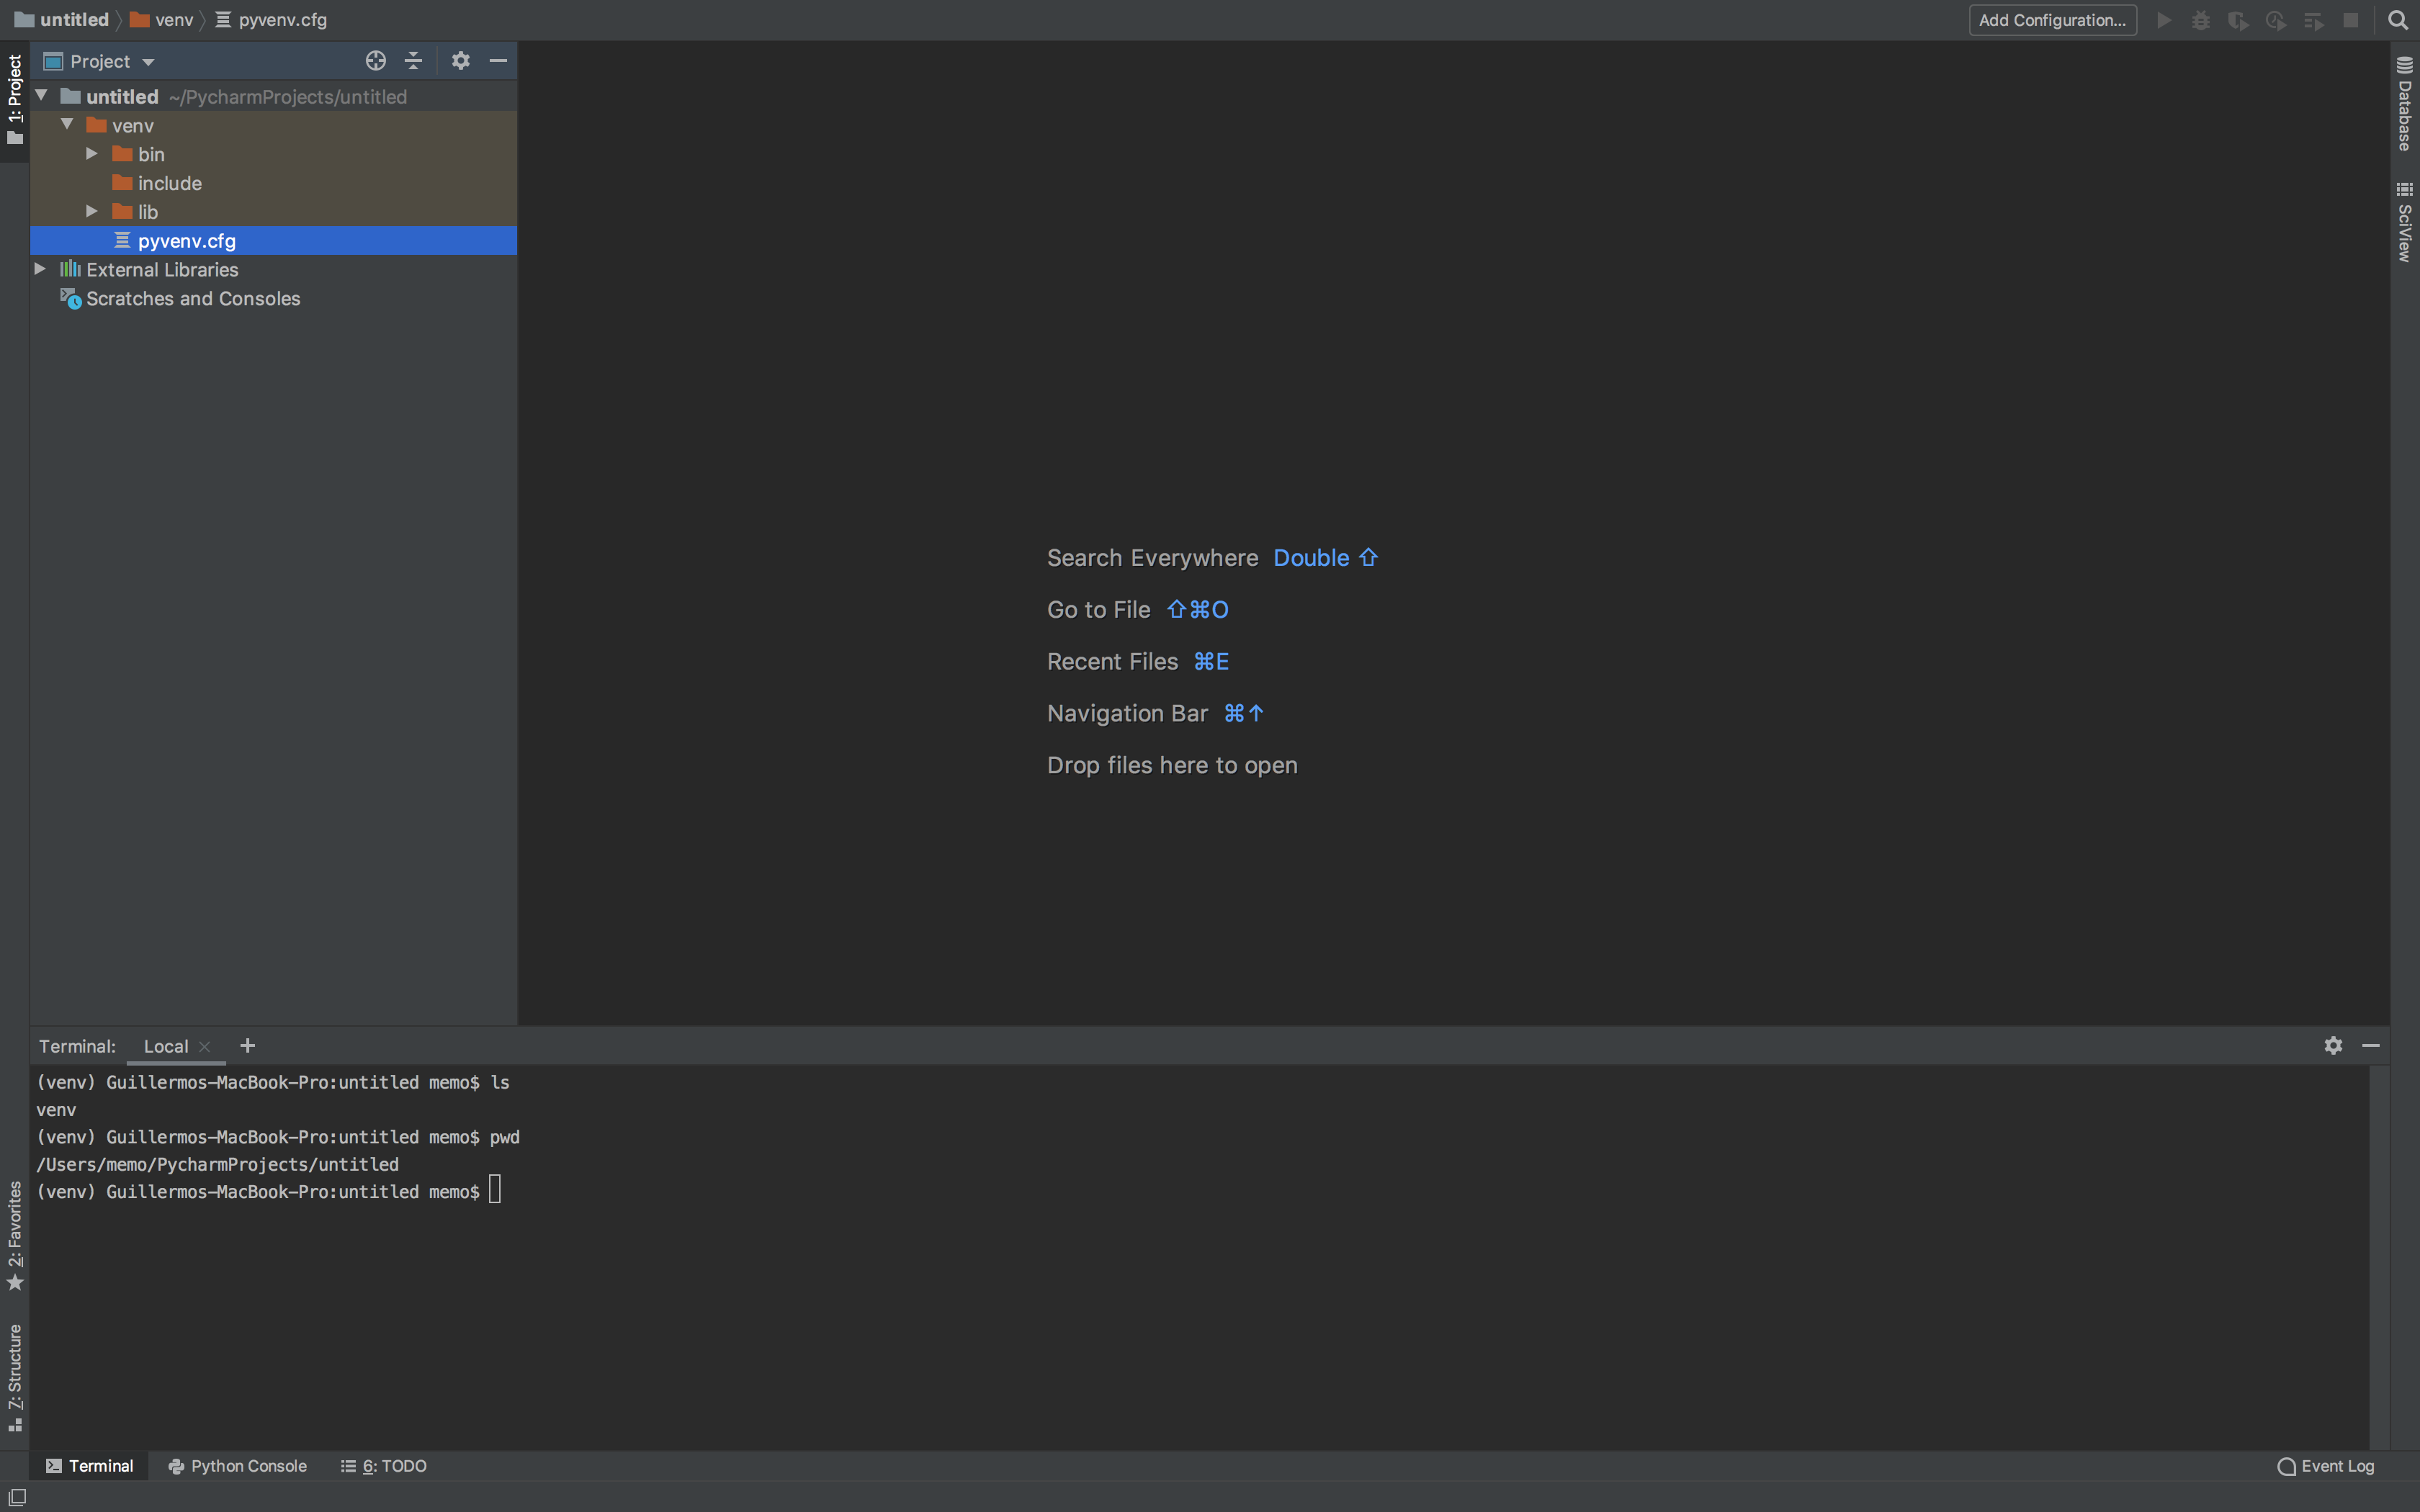
\includegraphics[width=0.85\linewidth]{pycharm_ide.png}
\end{frame}

%slide
\begin{frame}{First Complete-ish Developmental Environment}
\centering

\includegraphics[width=0.25\linewidth]{py.png} \hspace{1cm}

\includegraphics[width=0.23\linewidth]{pcharm.png} \hspace{1cm}
\pause

\includegraphics[width=0.17\linewidth]{mercurial.png}
\end{frame}

%slide
\begin{frame}{Upgrading the Workflow}
\centering

\includegraphics[width=0.27\linewidth]{dlogo.png} \hspace{2cm}
\pause

\includegraphics[width=0.22\linewidth]{atom.png}
\end{frame}

%slide
\begin{frame}{Atom IDE}
\centering
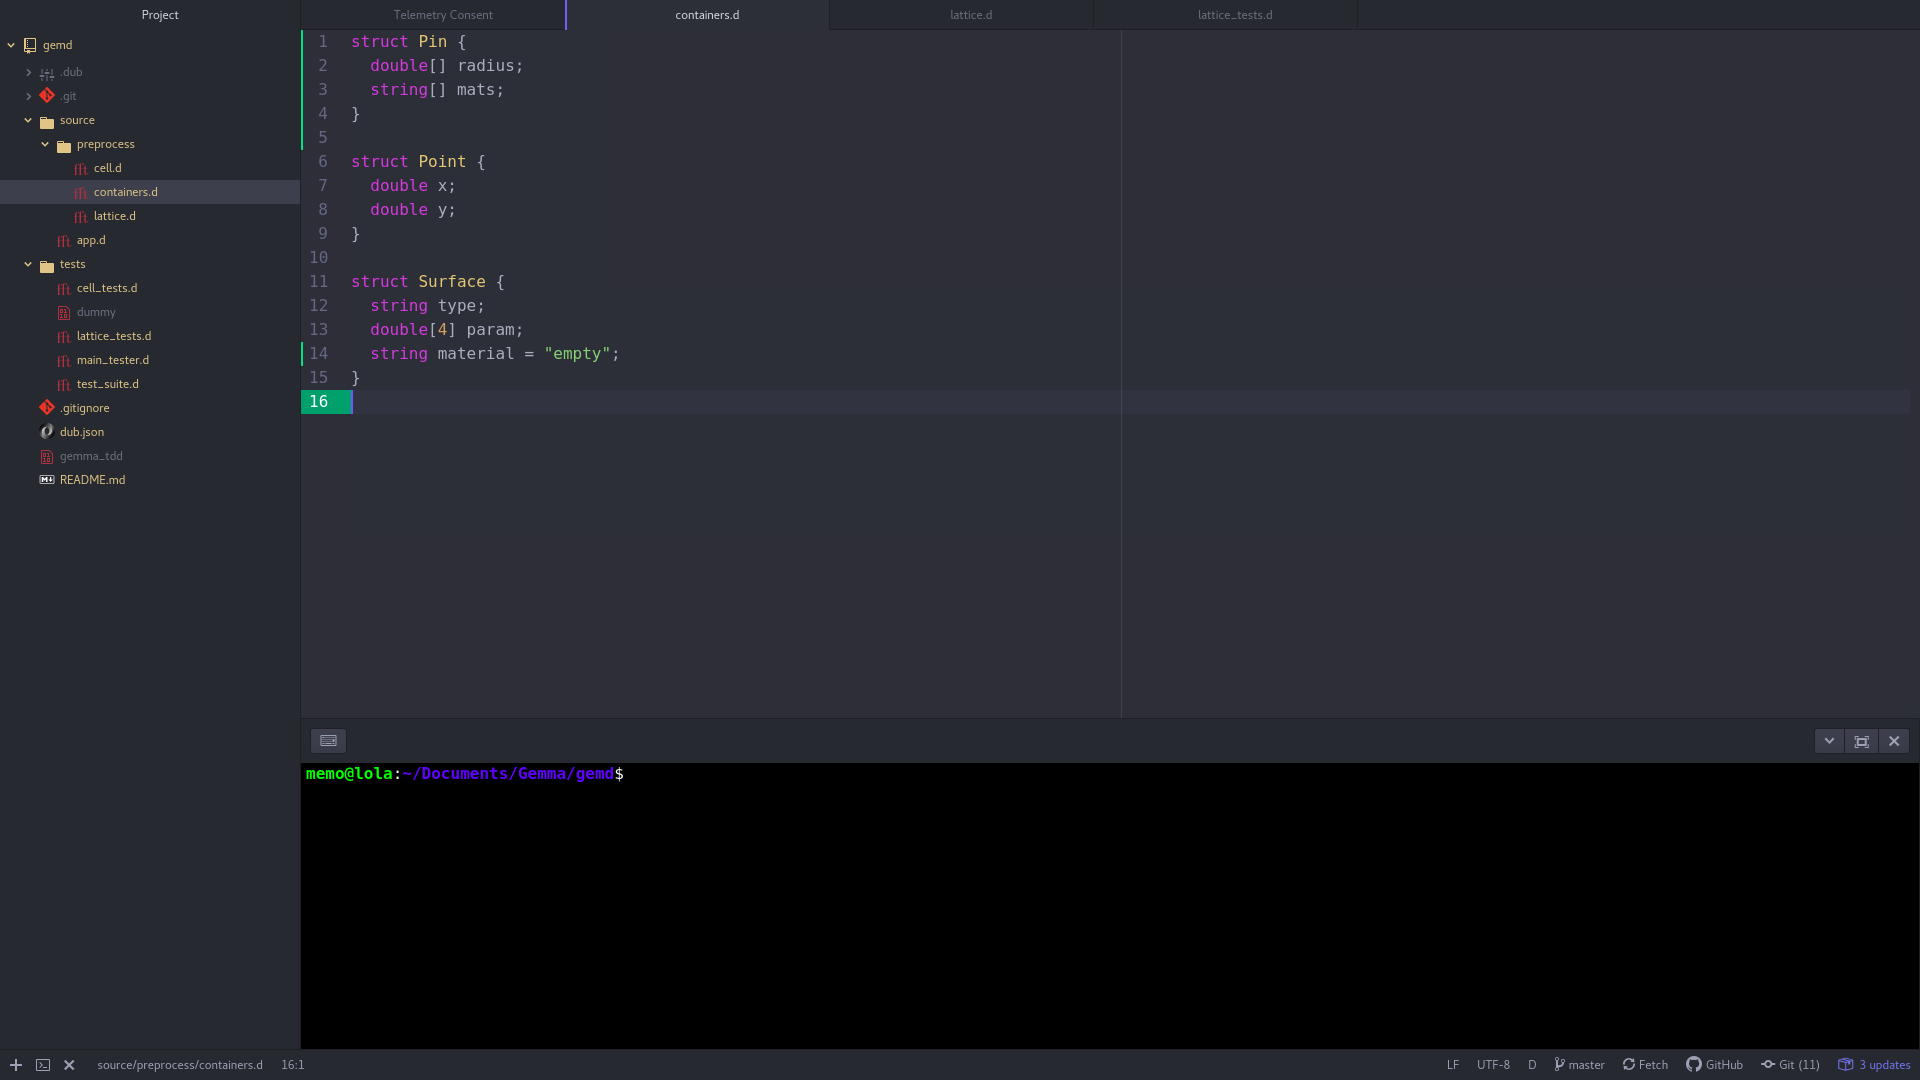
\includegraphics[width=0.85\linewidth]{atom_workflow.png}
\end{frame}

%slide
\begin{frame}{Cloud Repositories}
\centering

\includegraphics[width=0.30\linewidth]{github.png} \hspace{1cm}

\includegraphics[width=0.30\linewidth]{bitbucket.png}
\end{frame}

%slide
\begin{frame}{Git Basics}
  \centering
  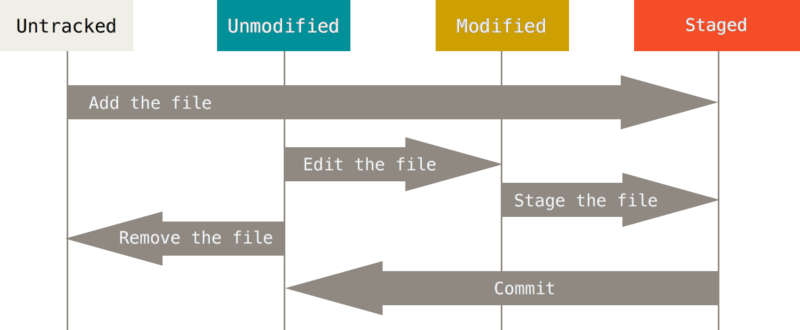
\includegraphics[width=0.85\linewidth]{lifecycle.png}
\end{frame}

%slide
\begin{frame}[fragile]{Git Basics - Checking file status}
  \begin{lstlisting}[frame=single, backgroundcolor=\color{gray!20}, basicstyle=\tiny]
  $ echo 'My Project' > README
  $ git status
  On branch master
  Your branch is up-to-date with 'origin/master'.
  Untracked files:
    (use "git add <file>..." to include in what will be committed)

      README

  nothing added to commit but untracked files present (use "git add" to track)
  \end{lstlisting}
\end{frame}

%slide
\begin{frame}[fragile]{Git Basics - Tracking New Files}
  \begin{lstlisting}[frame=single, backgroundcolor=\color{gray!20}, basicstyle=\tiny]
  $ git add README
  $ git status
  On branch master
  Your branch is up-to-date with 'origin/master'.
  Changes to be committed:
    (use "git restore --staged <file>..." to unstage)

      new file:   README
  \end{lstlisting}
\end{frame}

%slide
\begin{frame}[fragile]{Git Basics - Staging Modified Files}
  \begin{lstlisting}[frame=single, backgroundcolor=\color{gray!20}, basicstyle=\tiny]
  $ git status
  On branch master
  Your branch is up-to-date with 'origin/master'.
  Changes to be committed:
    (use "git reset HEAD <file>..." to unstage)

      new file:   README

  Changes not staged for commit:
    (use "git add <file>..." to update what will be committed)
    (use "git checkout -- <file>..." to discard changes in working directory)

      modified:   CONTRIBUTING.md
  \end{lstlisting}
  \pause
  \begin{lstlisting}[frame=single, backgroundcolor=\color{gray!20}, basicstyle=\tiny]
  $ git add CONTRIBUTING.md
  $ git status
  On branch master
  Your branch is up-to-date with 'origin/master'.
  Changes to be committed:
    (use "git reset HEAD <file>..." to unstage)

      new file:   README
      modified:   CONTRIBUTING.md
  \end{lstlisting}
\end{frame}

%slide
\begin{frame}[fragile]{Git Basics - Staging Modified Files...}
  \begin{lstlisting}[frame=single, backgroundcolor=\color{gray!20}, basicstyle=\tiny]
  $ vim CONTRIBUTING.md
  $ git status
  On branch master
  Your branch is up-to-date with 'origin/master'.
  Changes to be committed:
    (use "git reset HEAD <file>..." to unstage)

      new file:   README
      modified:   CONTRIBUTING.md

  Changes not staged for commit:
    (use "git add <file>..." to update what will be committed)
    (use "git checkout -- <file>..." to discard changes in working directory)

      modified:   CONTRIBUTING.md
  \end{lstlisting}
  \pause
  \begin{lstlisting}[frame=single, backgroundcolor=\color{gray!20}, basicstyle=\tiny]
  $ git add CONTRIBUTING.md
  $ git status
  On branch master
  Your branch is up-to-date with 'origin/master'.
  Changes to be committed:
    (use "git reset HEAD <file>..." to unstage)

      new file:   README
      modified:   CONTRIBUTING.md
  \end{lstlisting}
\end{frame}

%slide
\begin{frame}[fragile]{Git Basics - Short Status}
  \begin{lstlisting}[frame=single, backgroundcolor=\color{gray!20}, basicstyle=\tiny]
  $ git status -s
   M README
  MM Rakefile
  A  lib/git.rb
  M  lib/simplegit.rb
  ?? LICENSE.txt
  \end{lstlisting}
\end{frame}

%slide
\begin{frame}[fragile]{Git Basics - Ignoring Files}
  \begin{lstlisting}[frame=single, backgroundcolor=\color{gray!20}, basicstyle=\tiny]
  $ cat .gitignore
  *.[oa]
  *~
  \end{lstlisting}
  \pause
  \begin{lstlisting}[frame=single, backgroundcolor=\color{gray!20}, basicstyle=\tiny]
  $ cat .gitignore
  # ignore all .a files
  *.a

  # but do track lib.a, even though you're ignoring .a files above
  !lib.a

  # only ignore the TODO file in the current directory, not subdir/TODO
  /TODO

  # ignore all files in any directory named build
  build/

  # ignore doc/notes.txt, but not doc/server/arch.txt
  doc/*.txt

  # ignore all .pdf files in the doc/ directory and any of its subdirectories
  doc/**/*.pdf
  \end{lstlisting}
\end{frame}

%slide
\begin{frame}[fragile]{Git Basics - Removing Files}
  \begin{lstlisting}[frame=single, backgroundcolor=\color{gray!20}, basicstyle=\tiny]
  $ rm PROJECTS.md
  $ git status
  On branch master
  Your branch is up-to-date with 'origin/master'.
  Changes not staged for commit:
    (use "git add/rm <file>..." to update what will be committed)
    (use "git checkout -- <file>..." to discard changes in working directory)

          deleted:    PROJECTS.md

  no changes added to commit (use "git add" and/or "git commit -a")
  \end{lstlisting}
  \pause
  \begin{lstlisting}[frame=single, backgroundcolor=\color{gray!20}, basicstyle=\tiny]
  $ git rm PROJECTS.md
  rm 'PROJECTS.md'
  $ git status
  On branch master
  Your branch is up-to-date with 'origin/master'.
  Changes to be committed:
    (use "git reset HEAD <file>..." to unstage)

      deleted:    PROJECTS.md
  \end{lstlisting}
\end{frame}

%slide
\begin{frame}[fragile]{Git Basics - Committing}
  \begin{lstlisting}[frame=single, backgroundcolor=\color{gray!20}, basicstyle=\tiny]
  $ git commit
  # Please enter the commit message for your changes. Lines starting
  # with '#' will be ignored, and an empty message aborts the commit.
  # On branch master
  # Your branch is up-to-date with 'origin/master'.
  #
  # Changes to be committed:
  #	new file:   README
  #	modified:   CONTRIBUTING.md
  #
  ~
  ~
  ~
  ".git/COMMIT_EDITMSG" 9L, 283C
  \end{lstlisting}
  \pause
  \begin{lstlisting}[frame=single, backgroundcolor=\color{gray!20}, basicstyle=\tiny]
  $ git commit -m "Story 182: Fix benchmarks for speed"
  [master 463dc4f] Story 182: Fix benchmarks for speed
   2 files changed, 2 insertions(+)
   create mode 100644 README
  \end{lstlisting}
\end{frame}

%slide
\begin{frame}{Git Addons with Atom}
  \centering
  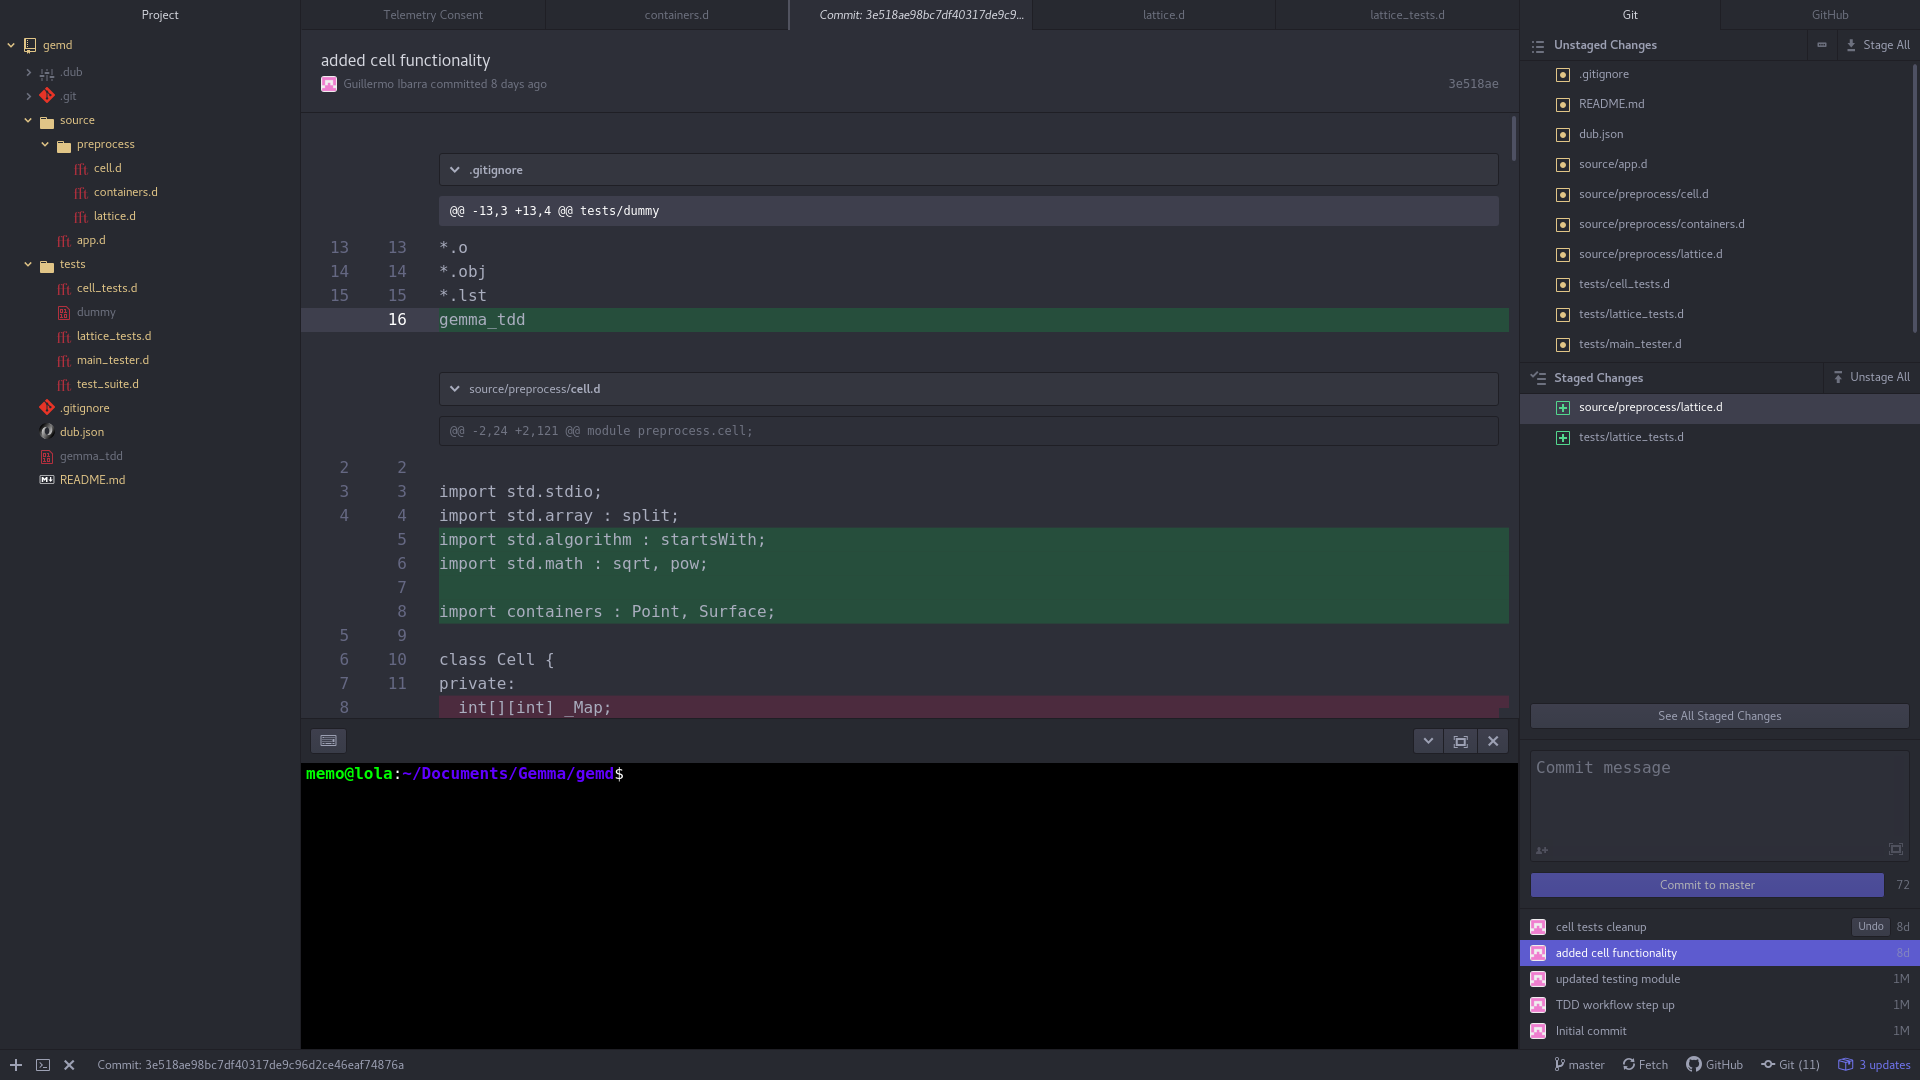
\includegraphics[width=0.85\linewidth]{git_atom.png}
\end{frame}

%slide
\begin{frame}{Tests? Tests!}
\centering
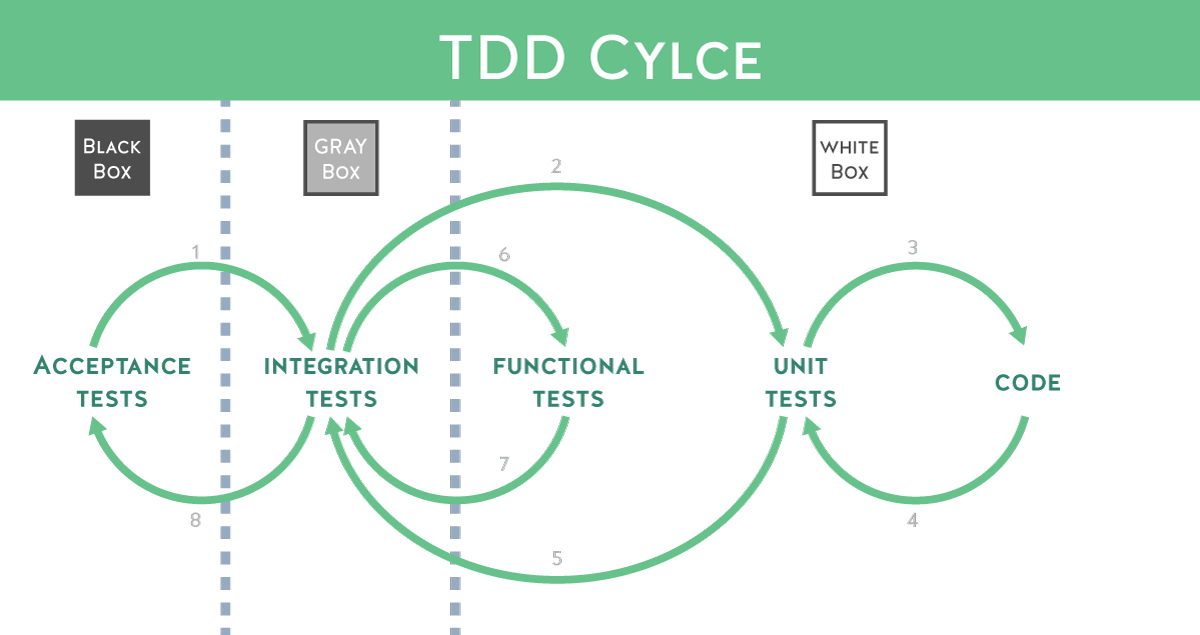
\includegraphics[width=0.85\linewidth]{tdd.png}
\end{frame}

%slide
\begin{frame}{Tests in Greater Detail}
\centering
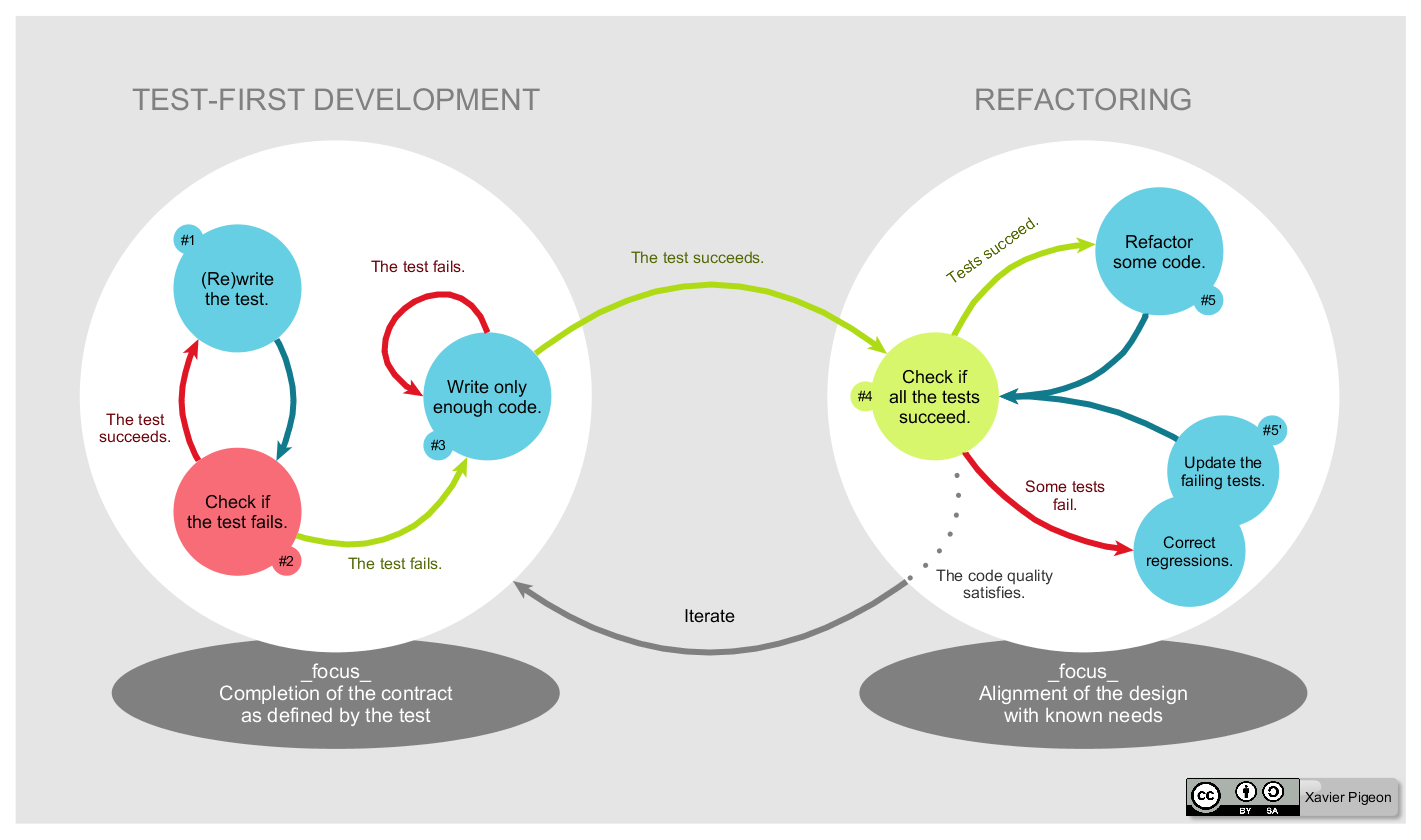
\includegraphics[width=0.85\linewidth]{tests.png}
\end{frame}

%slide
\begin{frame}[fragile]{Testing with D}
  \small
  Using DUB package manager, dub.json file:
  \begin{lstlisting}[frame=single, backgroundcolor=\color{background}, basicstyle=\tiny, keepspaces=true]
    {
      "name": "gemma_tdd",
      "description": "2D neutron transport solver, TDD D implementation",

      "authors": [ "Guillermo", "Samuel Vargas", "Hirepan Palomares"],
      "copyright": "Copyright  2020, Guillermo, Samuel Vargas, Hirepan Palomares",
      "license": "proprietary",

      "configurations": [
        {
          "name": "application",
          "targetType": "executable",
        },
        {
          "name": "unittest",
          "targetType": "executable",
          "targetPath": "tests",
          "targetName": "dummy",
          "mainSourceFile": "tests/main_tester.d",
          "excludedSourceFiles": ["source/app.d"],
          "sourcePaths": ["tests/"],
          "importPaths": ["tests/"]
        }
      ]
    }
  \end{lstlisting}
\end{frame}

%slide
\begin{frame}[fragile]{Testing Structure}
  \centering
  \begin{forest}
    for tree={font=\sffamily, grow'=0,
    folder indent=1em, folder icons,
    edge=densely dotted}
    [gemd
      [source]
      [tests
          [cell\_tests.d, is file]
          [lattice\_tests.d, is file]
          [main\_tester.d, is file]
          [test\_suite.d, is file]]
    ]
  \end{forest}
\end{frame}

%slide
\begin{frame}[fragile]{Compiling with DUB}
  \begin{lstlisting}[frame=single, backgroundcolor=\color{gray!20}, basicstyle=\tiny]
  $ dub build
  Performing "debug" build using /usr/bin/dmd for x86_64.
  gemma_tdd ~master: building configuration "application"...
  Linking...
  \end{lstlisting}
  \pause
  \begin{lstlisting}[frame=single, backgroundcolor=\color{gray!20}, basicstyle=\tiny]
  $ dub test
  Running custom 'unittest' configuration.
  Performing "unittest" build using /usr/bin/dmd for x86_64.
  gemma_tdd ~master: building configuration "unittest"...
  Linking...
  Running ./tests/dummy
  ----------------------------------------------------------------
                             T E S T S
  ----------------------------------------------------------------
  Running surfaceSpecificationTest()                        : PASS
  Running cellSpecificationTest()                           : PASS
  Running cellDimensionTest()                               : PASS
  Running pinConsistancyTest()                              : FAIL
  ----------------------------------------------------------------
  End of tests. Total: 4 Failed: 1
  \end{lstlisting}
\end{frame}

%slide
\begin{frame}{Code Documentation}
\centering

\includegraphics[width=0.40\linewidth]{dox.png} \hspace{1cm}
\pause

\includegraphics[width=0.30\linewidth]{sphinx.png}
\end{frame}

%slide
\begin{frame}{HPC Potential}
\centering

\includegraphics[width=0.30\linewidth]{intel.jpeg}
\end{frame}

%slide
\begin{frame}
\centering
\Huge
Thanks! \\
Questions?
\end{frame}

%slide
\begin{frame}{Extras}
  \begin{itemize}
    \item Git Manual \url{https://git-scm.com/book/en/v2}
    \item Git branch strategies \url{https://nvie.com/posts/a-successful-git-branching-model/}
    \item Test Driven Development \url{http://www.agiledata.org/essays/tdd.html}
  \end{itemize}
\end{frame}

\end{document}
